\section{Objectives}
Follow Lab 5 (PDF pages 21--23) to observe Miller coupling at the second stage of a three-inverter chain and quantify rail excursions and loading.

\section{Specification mapping}
\begin{longtable}{p{0.31\linewidth}p{0.29\linewidth}p{0.31\linewidth}}
\toprule
Handout requirement (PDF page) & Implementation & Verification and scope \\\midrule
Step 1: three inverters and stage-2 glitches (21--23) & 01\_miller, case 0 & Simulated with native parasitics \\
Step 2: add and vary $C_c$ (22--23) & Cases 1--3: 2/5/10 fF & Includes the specified 5 fF \\
Question: increase output load (23) & Cases 4--5: add 10/40 fF & Compare at fixed 5 fF coupling \\
\bottomrule
\end{longtable}


\section{Circuit and design derivation}
All three inverters use $W_n/W_p/L=0.6/1.8/0.25\,\mu$m. $C_c$ spans the second-stage input and output. Stage 3 remains a gate load, while additional $C_L$ connects to ground. The qualitative relation $\Delta V_o\approx C_c\Delta V_i/(C_c+C_{\rm out})$ explains charge division; nonlinear MOS simulation supplies the actual values. Scattered source cases are replaced by comparable parameter cases with explicit peak and edge measurements.

\section{Simulation setup}
This teaching rewrite uses a separately supplied model at 1.0 V and $25\,^{\circ}\mathrm C$. The specified topology, loads and comparative dimensions are retained. The handout's 2.5 V process results are not acceptance values for this model. The chosen 1 V is a simulation condition, not a verified device rating. MOS bulk terminals are explicitly connected to the corresponding supply rails.

HSPICE S-2021.09 uses RUNLVL=6, retaining waveforms, printed data and native measurements. Figures are redrawn from actual data; CSV files are in each Lab's results directory. Successful solution does not establish process reliability. Warnings from encrypted model blocks remain suppressed; the existing diagnostic did not expose actionable further details, so the warnings are not declared harmless and complete model-limit compliance is not claimed.

Input edges are 0.1 ns, with a 1 ns initial delay, 2 ns high interval and 5 ns period. Transient duration is 10 ns with 1 ps printing. Peaks are measured over 0.8--5 ns; rise/fall use 10--90\%/90--10\% crossings.

\section{Results and specification checks}
All six cases concluded normally without errors or failed measurements. $C_L$ is additional to the stage-3 gate load.
\begin{center}\small
\begin{tabular}{llllll}
\toprule
$C_c$ (fF) & $C_L$ (fF) & Over (mV) & Under (mV) & $t_r$ (ps) & $t_f$ (ps) \\
\midrule
0 & 0 & 123.09 & 83.47 & 133.70 & 76.70 \\
2 & 0 & 154.03 & 130.47 & 155.08 & 99.82 \\
5 & 0 & 188.80 & 182.72 & 189.49 & 133.95 \\
10 & 0 & 227.81 & 237.61 & 250.08 & 190.65 \\
5 & 10 & 143.98 & 142.61 & 279.78 & 178.15 \\
5 & 40 & 80.57 & 80.85 & 558.95 & 318.36 \\
\bottomrule
\end{tabular}
\end{center}

\begin{figure}[htbp]
\centering
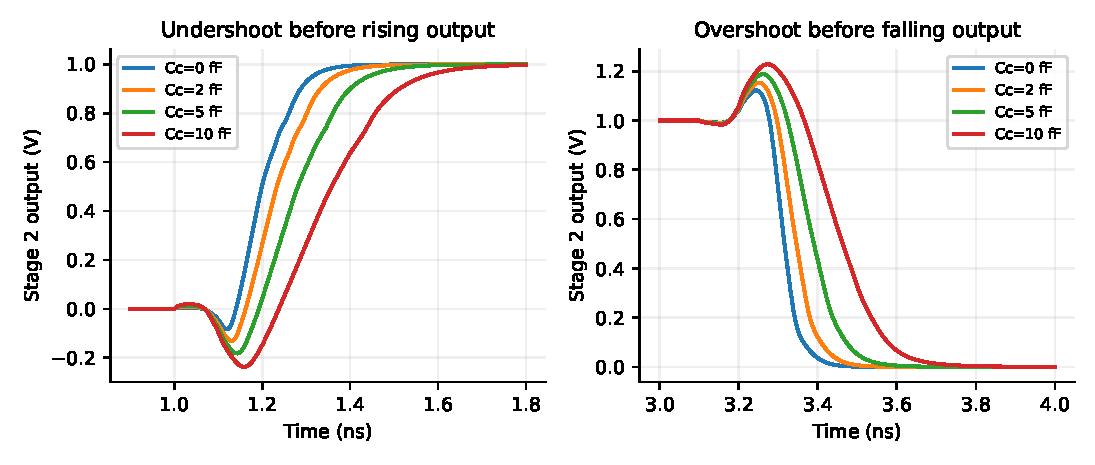
\includegraphics[width=\linewidth]{figures/miller_waveforms.pdf}
\caption{Transitions and rail excursions at stage 2; redrawn from this run's HSPICE data.}
\end{figure}

\begin{figure}[htbp]
\centering
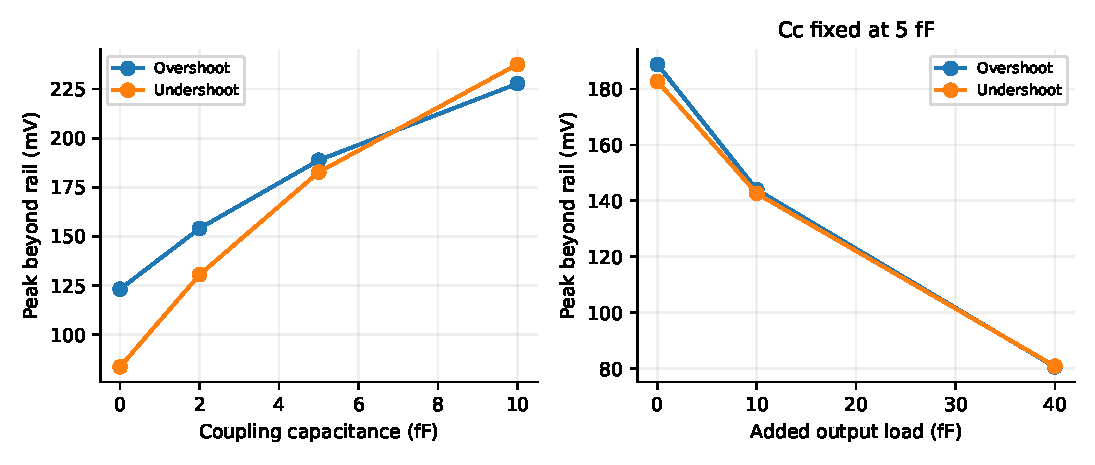
\includegraphics[width=\linewidth]{figures/miller_load_comparison.pdf}
\caption{Effect of coupling capacitance and additional output load; redrawn from this run's HSPICE data.}
\end{figure}


\section{Discussion}
Increasing $C_c$ from 0 to 10 fF raises overshoot from 123.09 to 227.81 mV and undershoot from 83.47 to 237.61 mV. At 5 fF coupling, adding 40 fF load reduces the peaks to about 80.6/80.9 mV while increasing rise/fall times to 559/318 ps. Zero added coupling does not remove intrinsic Miller capacitance. Rail excursions are simulation results; they do not establish hardware reliability or immunity of every receiver.

\section{Conclusion}
Both experimental steps and the loading question are covered by actual data. Results support capacitive coupling and charge-division reasoning under the stated model and stimulus.
